\chapter{Filtri per mastering}

\section{Introduzione}

\begin{itemize}
    \item Idealmente, la risposta in frequenza netta di un sistema dovrebbe essere uniforme per tutte le frequenze: da qui deriva il termine ``equalizzazione''.
    
    \item Il termine ``equalizzazione'' è stato utilizzato per indicare qualsiasi procedura che comporti l'alterazione o la regolazione della risposta in frequenza dell’ampiezza di un segnale.
    
    \item Il concetto di filtraggio delle frequenze audio è noto almeno fin dagli anni '70 del XIX secolo, ed è stato applicato nei primi progetti di telegrafi armonici.
    
    \item Le linee telefoniche venivano equalizzate nei ripetitori utilizzando filtri d'onda per annullare le risonanze causate da disadattamenti di impedenza o dall'attenuazione delle alte frequenze nei cavi lunghi.
    
    \item Il termine ``filtro'' può assumere numerosi significati. Un filtro seleziona le componenti del segnale in base alle frequenze che si desidera rifiutare, mantenere o enfatizzare.
    
    \item I filtri sono comunemente descritti nel dominio della frequenza, ma hanno anche effetti significativi nel dominio del tempo.
    
    \item Oltre alla loro funzione di modulazione della frequenza, i filtri possono essere analizzati nel dominio temporale, dando origine a una famiglia di effetti audio basati sul ritardo, come quelli che si possono sperimentare negli spazi acustici.
\end{itemize}

\section{Filtri base}

\begin{itemize}
    \item \textbf{Filtri passa-basso (LP)}: selezionano le basse frequenze fino alla frequenza di taglio $f_c$ e attenuano le frequenze superiori a $f_c$. Inoltre, una risonanza può amplificare le frequenze intorno a $f_c$.

    \item \textbf{Filtri passa-alto (HP)}: selezionano le frequenze superiori a $f_c$ e attenuano quelle inferiori, con la possibilità di una risonanza attorno a $f_c$.

    \item \textbf{Filtri passa-banda (BP)}: selezionano le frequenze comprese tra una frequenza di taglio inferiore $f_{cl}$ e una superiore $f_{ch}$.

    \item \textbf{Filtri bandreject (BR)}: attenuano le frequenze comprese tra $f_{cl}$ e $f_{ch}$, lasciando passare quelle al di fuori di questo intervallo.

    \item \textbf{Filtri all-pass}: permettono il passaggio di tutte le frequenze, ma modificano la fase del segnale in ingresso.
\end{itemize}


\begin{itemize}
    \item Il filtro passa-basso con risonanza è molto utilizzato nella computer music per simulare una struttura acustica risonante.

    \item Il filtro passa-alto è utile per rimuovere frequenze molto basse indesiderate.

    \item Il passa-banda può produrre effetti come l'imitazione di una linea telefonica o di una sordina applicata a uno strumento acustico.

    \item Il bandreject può dividere lo spettro udibile in due bande che risultano percepite come non correlate.
\end{itemize}

\section{Filtri canonici}

\begin{itemize}
    \item Esistono diversi modi per implementare un filtro. Il più semplice è il filtro canonico, spesso utilizzato per realizzare filtri del secondo ordine mediante equazioni alle differenze.
    
    \begin{figure}[H]
        \centering
        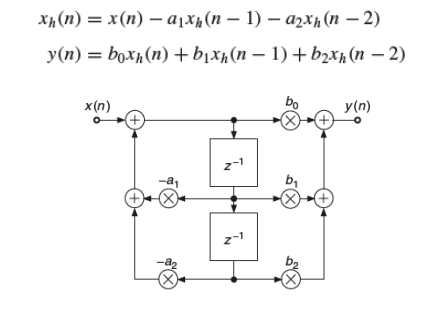
\includegraphics[width=0.7\textwidth]{capitoli/capitolo15/immagini/image1.png}
    \end{figure}
    

    \item A seconda dei coefficienti $a$ e $b$, si possono ottenere diversi comportamenti del filtro. Da tali coefficienti si ottiene la funzione di trasferimento del sistema.
    
    \begin{figure}[H]
        \centering
        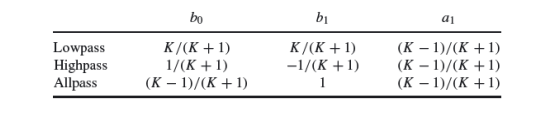
\includegraphics[width=0.7\textwidth]{capitoli/capitolo15/immagini/image2.png}
    \end{figure}

    \item Impostando $a_2 = b_2 = 0$, il filtro si riduce a un filtro del secondo ordine. Questo può essere utilizzato per implementare un filtro passa-tutto, passa-basso o passa-alto, con i coefficienti forniti in apposite tabelle. Il parametro $K$ dipende dalla frequenza di taglio.
    
    \item Nel filtro passa-tutto, il coefficiente $K$ controlla anche la frequenza $f_c$ alla quale si raggiunge uno sfasamento di $-90^\circ$.
\end{itemize}


\begin{itemize}
    \item Per i filtri del secondo ordine, oltre alla frequenza di taglio (o frequenza centrale), è necessario specificare anche il fattore $Q$, che assume significati diversi a seconda del tipo di filtro:
    
    \begin{itemize}
        \item Nei filtri passa-basso e passa-alto, $Q$ controlla l'altezza della risonanza. Per $Q = \frac{1}{\sqrt{2}}$, il filtro risulta massimamente piatto fino alla frequenza di taglio. Per valori inferiori di $Q$, si ha una maggiore attenuazione in banda passante; per valori superiori, si osserva un'amplificazione attorno a $f_c$.
        
        \item Nei filtri passa-banda e bandreject, $Q$ è legato alla larghezza di banda $f_b$ secondo la relazione $Q = \frac{f_c}{f_b}$, ovvero è l'inverso della larghezza di banda relativa $\frac{f_b}{f_c}$.
        
        \item Nel filtro passa-tutto, $Q$ controlla anch'esso la larghezza di banda, che in questo caso è definita dai punti in cui si raggiungono $\pm 90^\circ$ di sfasamento, rispetto ai $-180^\circ$ raggiunti in corrispondenza di $f_c$.
    \end{itemize}
    
    \item Sebbene i filtri canonici siano relativamente semplici dal punto di vista concettuale, il calcolo dei loro coefficienti a partire da parametri come la frequenza di taglio e la larghezza di banda può risultare complesso.
\end{itemize}

\begin{figure}[H]
    \centering
    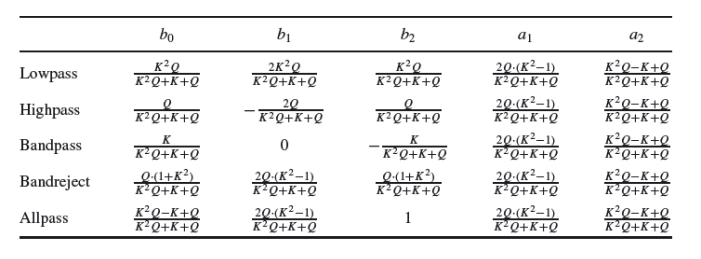
\includegraphics[width=0.7\textwidth]{capitoli/capitolo15/immagini/image3.png}
\end{figure}

\section{State Variable Filter}

\begin{itemize}
    \item Un'interessante alternativa alla struttura del filtro canonico è il \textit{filtro a variabili di stato}, che combina filtri passa-basso, passa-banda e passa-alto del secondo ordine, mantenendo la stessa frequenza di taglio $f_c$ e lo stesso fattore di qualità $Q$.

    \begin{figure}[H]
        \centering
        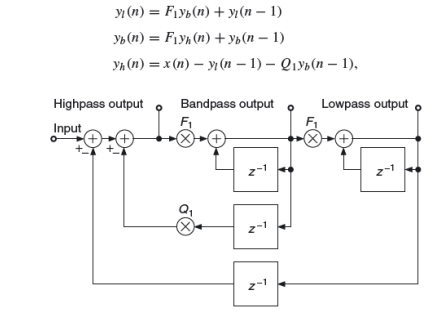
\includegraphics[width=0.7\textwidth]{capitoli/capitolo15/immagini/image4.png}
    \end{figure}

    \item I coefficienti di sintonizzazione $F_1$ e $Q_1$ sono correlati ai parametri $f_c$ e $Q$.

    \item Si può dimostrare che le funzioni di trasferimento per i tre tipi di filtro (passa-basso, passa-banda e passa-alto) dipendono dai parametri $r = F_1$ e $q = 1 - F_1 Q_1$.
\end{itemize}
\begin{figure}[H]
    \centering
    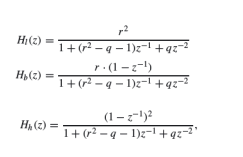
\includegraphics[width=0.3\textwidth]{capitoli/capitolo15/immagini/image5.png}
\end{figure}

\begin{itemize}
    \item Questa struttura è particolarmente efficace non solo nel processo di filtraggio, ma soprattutto per la semplicità delle relazioni tra i parametri di controllo e i coefficienti di sintonizzazione.

    \item È necessario considerare la stabilità del filtro: a frequenze di taglio elevate e per valori di $Q$ molto piccoli, il filtro può diventare instabile.

    \item Per garantire il funzionamento stabile del filtro a variabili di stato, è utile rispettare il limite di utilizzabilità dato dalla condizione:
    
    \[
    F_1 < 2 - Q_1
    \]

    \item Le proprietà di questo filtro sono state sfruttate in applicazioni creative, ad esempio per produrre glissandi infiniti a partire da suoni naturali, oppure per permettere transizioni fluide tra configurazioni estreme.
\end{itemize}

\section{Filtri all-pass}

\begin{itemize}
    \item Un filtro all-pass ha un comportamento piatto come risposta in frequenza del modulo.

    \item Può essere descritto come segue:

    \[
    H(s) = \frac{b(s)}{a(s)}
    \]

    dove $b(s)$ e $a(s)$ sono polinomi in $s$.

    \item Il filtro all-pass corrisponde a uno schema a blocchi del tipo:

    \begin{figure}[H]
        \centering
        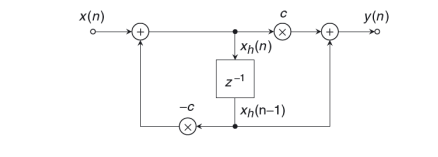
\includegraphics[width=0.7\textwidth]{capitoli/capitolo15/immagini/image6.png}
    \end{figure}
\end{itemize}


\begin{itemize}
    \item Dai filtri all-pass, combinando opportunamente gli elementi, è possibile derivare altre tipologie di filtro.
    
    \item La funzione di trasferimento di un filtro all-pass del secondo ordine è data da:

    \begin{figure}[H]
        \centering
        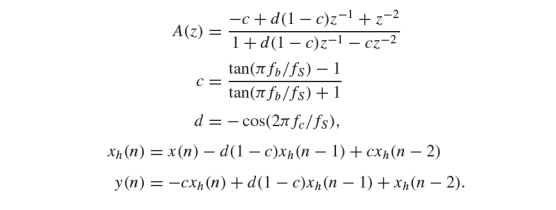
\includegraphics[width=0.7\textwidth]{capitoli/capitolo15/immagini/image7.png}
    \end{figure}

    dove $\zeta$ è il fattore di smorzamento e $\omega_n$ è la frequenza centrale.

    \item Il parametro $d$ regola la frequenza centrale e il parametro $c$ la larghezza di banda.
\end{itemize}

\bigskip

\begin{itemize}
    \item Gli all-pass del secondo ordine possono essere utilizzati per implementare in maniera efficace filtri passa-banda (BP) e bandreject (BR).
\end{itemize}

\section{FIR filters}

\begin{itemize}
    \item I filtri digitali che abbiamo visto in precedenza hanno una risposta all'impulso infinita.
    
    \item Al contrario, la risposta all’impulso per i filtri FIR è di durata finita.
    
    \item Questi filtri consentono di costruire tipi di filtro sofisticati, dove è necessaria una forte attenuazione delle frequenze indesiderate o la scomposizione del segnale in diverse bande di frequenza.
\end{itemize}

\section{FIR Comb filters(DOMANDA CERTA ALL'ESAME)}

\begin{itemize}
    \item Il segnale di ingresso viene ritardato di un determinato tempo. L'effetto sarà udibile solo quando il segnale elaborato viene combinato (aggiunto) al segnale di ingresso, che funge da riferimento. Questo effetto ha due parametri di regolazione:
    
    \begin{itemize}
        \item L'entità del ritardo $\tau$.
        
        \item L'ampiezza relativa del segnale ritardato rispetto a quella del segnale di riferimento.
    \end{itemize}
\end{itemize}

\begin{figure}[H]
    \centering
    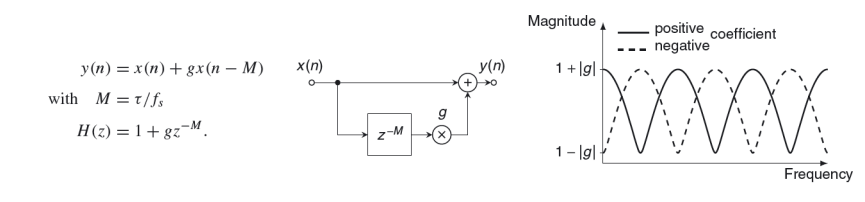
\includegraphics[width=0.7\textwidth]{capitoli/capitolo15/immagini/image8.png}
\end{figure}

\section{IIR Comb filters}

\begin{itemize}
    \item Imitando le infinite riflessioni alle due estremità di un cilindro, il filtro comb IIR produce una serie infinita di risposte $y(n)$ a un ingresso $x(n)$.
    
    \item Il segnale d'ingresso circola in una linea di ritardo che viene reintrodotta in ingresso.
\end{itemize}

\begin{figure}[H]
    \centering
    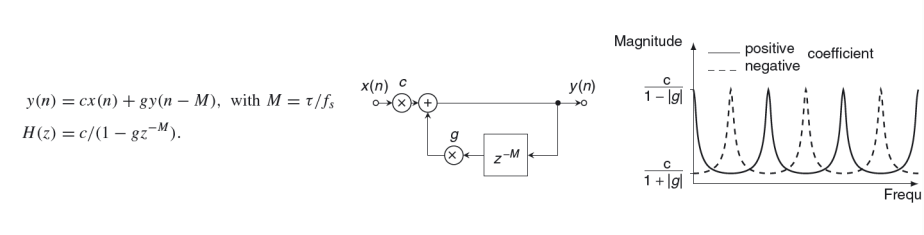
\includegraphics[width=0.7\textwidth]{capitoli/capitolo15/immagini/image9.png}
\end{figure}

\section{Universal Comb filters}

\begin{itemize}
    \item La combinazione dei filtri comb FIR e IIR conduce al filtro comb universale.
    
    \item Questa struttura di filtro si trasforma in una struttura all-pass nel caso speciale di $-BL = FB$, $FF = 1$, dove il ritardo a un campione $z^{-1}$ è sostituito dal ritardo a $M$ campioni $z^{-M}$.
\end{itemize}

\section{Shelving filters (I order)}

\begin{itemize}
    \item In maniera simile ai filtri LP/HP che possono essere costruiti partendo da degli all-pass, si possono ottenere filtri shelving del primo ordine partendo da all-pass del primo ordine con funzione di trasferimento $A(z)$.
\end{itemize}

\begin{itemize}
    \item I parametri di Cutoff boost ($C_b$) e Cutoff cut ($C_c$) variano a seconda del tipo di shelving filter desiderato:
    \begin{figure}[H]
        \centering
        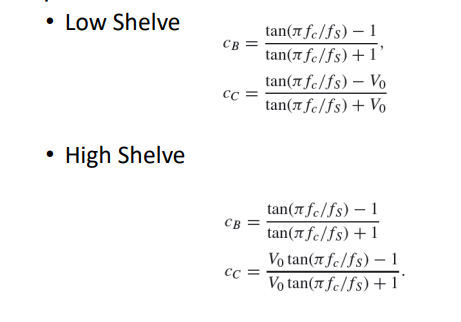
\includegraphics[width=0.7\textwidth]{capitoli/capitolo15/immagini/image10.png}
    \end{figure}
\end{itemize}
\vspace{5cm}
\section{Shelving filters (II order)}

\begin{itemize}
    \item Per diverse applicazioni, la pendenza del filtro shelving viene ulteriormente aumentata da funzioni di trasferimento di secondo ordine o superiore.
    
    \item Esistono diversi approcci per progettare filtri shelving di ordine superiore con un calcolo relativamente semplice dei coefficienti, al costo di strutture di filtro leggermente più complicate.
\end{itemize}
\begin{figure}[H]
    \centering
    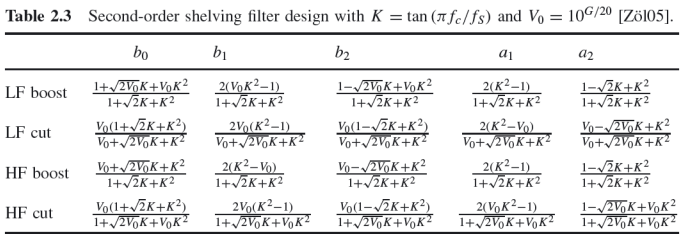
\includegraphics[width=0.7\textwidth]{capitoli/capitolo15/immagini/image11.png}
\end{figure}

\section{Peak filters}

\begin{itemize}
    \item In maniera analoga, un filtro peak del secondo ordine può essere derivato sfruttando un all-pass del secondo ordine.
\end{itemize}
\begin{figure}[H]
    \centering
    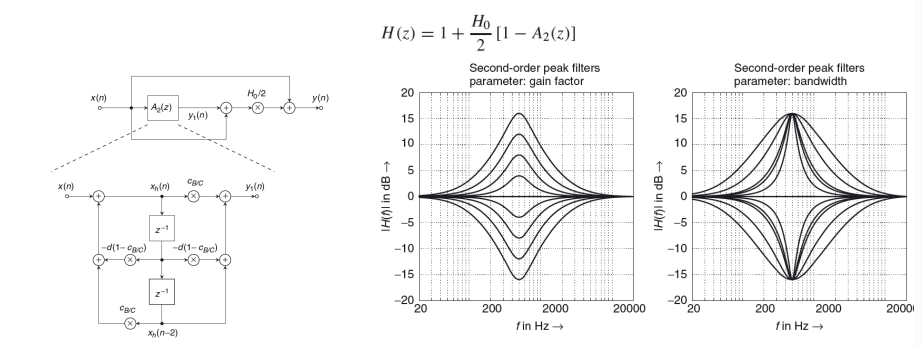
\includegraphics[width=0.7\textwidth]{capitoli/capitolo15/immagini/image12.png}
\end{figure}
\vspace{8cm}
\section{EQ}

\begin{itemize}
    \item A differenza dei filtri passa-basso/alto e passa/elimina-banda, che attenuano lo spettro audio al di sopra o al di sotto di una frequenza di taglio, gli equalizzatori modellano lo spettro audio modificando alcune bande di frequenza mentre altre rimangono inalterate.
    
    \item In genere, gli equalizzatori sono costruiti con un collegamento in serie di filtri shelving e di picco del primo e del secondo ordine, controllati in modo indipendente.
\end{itemize}

\section{GEQ (equalizzatori grafici)}

\begin{itemize}
    \item L'equalizzatore grafico è uno strumento che consente di regolare in modo indipendente il guadagno di più regioni di frequenza in un segnale audio.
    
    \item I comuni equalizzatori grafici possono fornire fino a circa 30 controlli per la manipolazione della risposta in frequenza di ciascun canale audio.
    
    \item Strutturalmente, un equalizzatore grafico è un insieme di filtri, ciascuno con una frequenza centrale e una larghezza di banda fisse. L'unico controllo da parte dell'utente è il guadagno di comando, ovvero la quantità di incremento o di taglio in ciascuna banda di frequenza.
\end{itemize}

\bigskip

\begin{itemize}
    \item Il guadagno di ciascuna banda di frequenza può essere solitamente regolato entro un intervallo di 12 dB, corrispondente a circa $0.25 < G < 4$ per ciascun filtro.
    
    \item Il termine \textit{grafico} si riferisce al fatto che la posizione delle manopole dei cursori può essere intesa come un grafico della risposta in magnitudine dell'equalizzatore.
    
    \item Un equalizzatore grafico può essere implementato utilizzando una cascata di filtri equalizzatori o un banco parallelo di filtri passa-banda.
    
    \item In un'implementazione a cascata, ogni filtro determina la risposta intorno alla frequenza centrale in base al proprio guadagno (peak filters, guadagno 1 fuori banda).
    
    \item In un'implementazione parallela, ogni filtro passa-banda produce alla sua frequenza centrale un guadagno determinato dal guadagno del suo comando (BP filters, guadagno –inf fuori banda).
\end{itemize}
